%{\let\clearpage\relax \chapter*{Содержание работы}}
%\section*{Содержание работы}
\chapter*{Содержание работы}
В данной работе описывается разработка физической модели нового высокопроизводительного метода формирования трехмерных микро- и наноструктур -- сухого электронно-лучевого травления резиста (СЭЛТР). 

В начале \underline{\textbf{первой главы}} приводится описание основных методов микро- и наноструктурирования, существующих в настоящее время. Исходя из их преимуществ и недостатков делается заключение о том, что в настоящее время отсутствует метод формирования произвольных трехмерных структур, который являлся бы одновременно высокопроизводительным и относительно простым в реализации.

Далее рассматривается концепция микролитографии на основе локальной электронно-стимулированной термической деполимеризации резиста и описываются первые шаги в разработке метода СЭЛТР.
Проведенные в работе~\cite{Bruk_2016_mee} эксперименты демонстрируют высокую производительность данного метода, а также сглаженный профиль получаемых структур (рисунок~\ref{fig:DEBER_many_profiles}).
При этом в работе отмечается низкое латеральное разрешение метода СЭЛТР, значительно ограничивающее область его применения.
Поскольку в методе СЭЛТР профиль линии формируется под действием нескольких одновременно протекающих процессов, определение влияния каждого из них на результирующий профиль, выявление путей оптимизации метода и оценка его возможностей на основе лишь экспериментальных исследований представлялись затруднительными.
Основные процессы, протекающие при СЭЛТР, по отдельности являются относительно хорошо изученными, но их совместное протекание в процессе микроструктурирования до настоящего момента не исследовалось.
Таким образом, целесообразным являлось создание физической модели сухого электронно-лучевого травления резиста, которая позволила бы определить предельное разрешение метода СЭЛТР, а также оценить возможность его применения для формирования различных необходимых структур.
\begin{figure}
	\centering
	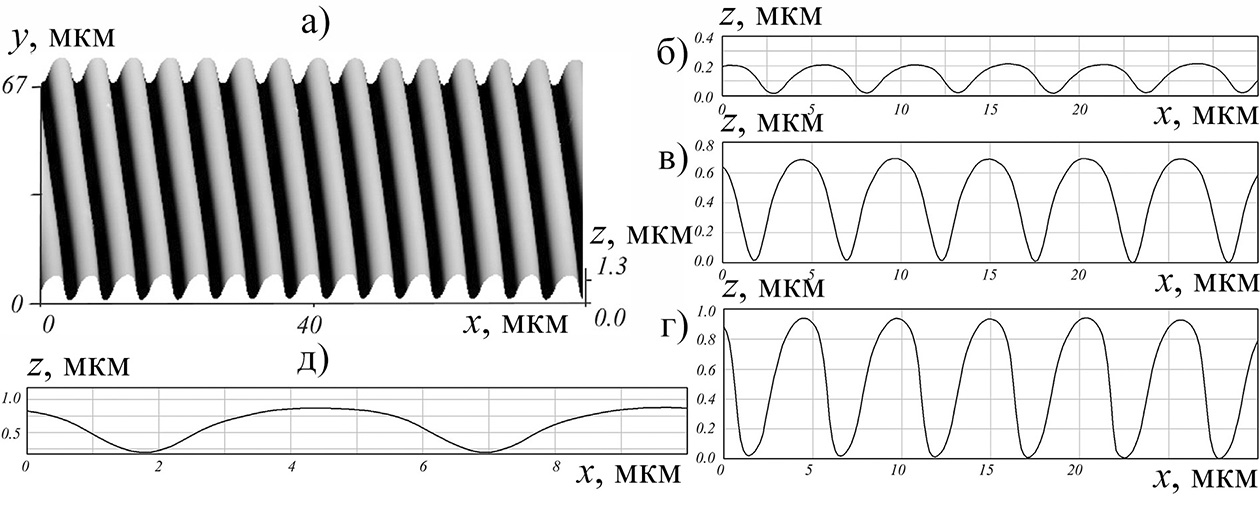
\includegraphics{1_chapter/DEBER_many_profiles_14pt_200}
	\vspace{0.2em}
	\caption{Профили периодических структур, полученных методом СЭЛТР в слое ПММА толщиной 900 нм при экспонировании вдоль серии параллельных линий при температуре 160~$^\circ$C: а) трехмерное изображение; б), в), г) профили, полученные при дозах экспонирования 0.05, 0.2 и 0.87 мкКл/см$\pp$ соответственно; д) изображение профиля в) в масштабе 1:1~\cite{Bruk_2016_mee}.}
	\label{fig:DEBER_many_profiles}
\end{figure}

\underline{\textbf{Вторая глава}} посвящена описанию существующих моделей и методов моделирования процессов, протекающих при СЭЛТР.
Основными процессами, влияющими на профиль линии в методе СЭЛТР, являются рассеяние электронного пучка в резисте и подложке, электронно-стимулированные разрывы молекул резиста, электронно-стимулированная термическая деполимеризация резиста, диффузия мономера и растекание резиста.
Некоторые из этих процессов достаточно хорошо изучены -- так, в настоящее время существуют высокоточные модели упругого и неупругого рассеяния электронного пучка в веществе.
В то же время, некоторые процессы являются изученными относительно слабо -- например, для описания электронно-стимулированных разрывов молекул резиста существует только макроскопический подход, основанный на анализе распределения энергии, выделившейся в слое резисте~\cite{Greeneich1979_Mf_Mn}.
Кинетические модели термической деполимеризации полимеров, в свою очередь, требуют задания различных констант, значения которых приведены в литературе лишь для некоторых частных случаев~\cite{Boyd_3, Mita_PMMA_zip_lengths_T}.
В отдельную группу можно выделить процессы диффузии мономера и растекания резиста -- для них существуют простые и в то же время достаточно точные модели~\cite{Fragala_3_diffusion, Leveder_2010, Kirchner_reflow}, однако, эти модели не могут быть использованы в исходном виде в силу неоднородности резиста в методе СЭЛТР.
Таким образом, для описания процессов, протекающих при сухом электронно-лучевом травлении резиста, требуется существенная доработка существующих моделей либо разработка на их основе новых моделей.

В \underline{\textbf{третьей главе}} описываются методы, которые использовались при разработке и верификации модели сухого электронно-лучевого травления резиста.
В соответствии с проведенными ранее экспериментами в данной работе в качестве резиста был выбран полиметилметакрилат (ПММА), в качестве материала подложки -- кремний~(Si).

Для моделирования рассеяния электронного пучка в системе ПММА/Si был реализован алгоритм на основе метода Монте-Карло. Для описания упругих процессов использовались моттовские сечения упругого рассеяния, сечения неупругого электрон-электронного рассеяния рассчитывались из функций потерь энергии ПММА и кремния.
Для повышения точности моделирования также учитывались неупругие процессы электрон-фононного и электрон-поляронного рассеяния в слое ПММА~\cite{Ciappa_2010}.

Для моделирования электронно-стимулированных разрывов молекул ПММА при повышенной температуре была разработана оригинальная микроскопическая модель.
В качестве приводящих к разрыву полимерных молекул в ней рассматривались процессы электрон-электронного рассеяния, и для моделирования электронно-стимулированных разрывов молекул ПММА была введена вероятность разрыва при электрон-электронном рассеянии $\ps$.
При заданной вероятности разрыва $\ps$ акты электрон-электронного рассеяния, приводящие к разрыву молекул, моделировались методом Монте-Карло:
\begin{equation} \label{eq:MC_9}
	\begin{aligned}
		\xi < \ps & \Rightarrow \text{разрыв молекулы} \\
		\xi \geq \ps & \Rightarrow \text{нет разрыва},
	\end{aligned}
\end{equation}
где $\xi$ -- случайное число из промежутка [0, 1).
Значения $\ps$ для различных температур были найдены путем моделирования эксперимента по вычислению радиационно-химического выхода разрывов молекул ПММА $\Gs$.
Значение $\Gs$, определяемое как число разрывов молекул, происходящих при выделении в слое полимерного резиста энергии 100~эВ, вычисляется экспериментально на основе значений среднечисловой молекулярной массы резиста до и после экспонирования~\cite{Greeneich1979_Mf_Mn}.
Для моделирования экспериментального значения $\Gs$ сначала на основе модели идеальной цепи проводилось моделирование слоя ПММА.
Далее моделировались акты электрон-электронного рассеяния, которые впоследствии сопоставлялись конкретным мономерам в модели слоя ПММА.
Это позволило при каждом значении $\ps$ промоделировать распределение молекулярной массы ПММА после экспонирования и затем промоделировать экспериментальное значение $\Gs$.
Так, для каждой температуры было подобрано значение $\ps$, обеспечивающее соответствие между промоделированным и экспериментальным~\cite{Charlesby_1964_Gs} значениями $\Gs$.
Было установлено, что экспериментально зарегистрированное увеличение $\Gs$ ростом температуры от 0 до 200~$^\circ$C может быть описано за счет увеличения вероятности разрыва молекулы ПММА при электрон-электронном рассеянии от 0.045 до 0.105.

Для моделирования электронно-стимулированной термической деполимеризации ПММА в процессе СЭЛТР использовалась кинетическая модель термической деполимеризации при возникновении активных центров деполимеризации в произвольных точках внутри полимерной молекулы~\cite{Boyd_3}.
В случае постоянной концентрации радикализованных молекул эта модель приводит к системе уравнений вида
%\begin{equation} \label{eq:moment_equation}
%	\frac{d M_i}{d t}=k_s\left(\frac{2}{i+1}-1\right) M_{i+1}+\frac{d M_0}{d t}-k_s M_1 - \frac{i}{\gamma}\left(k_s M_i+\frac{d M_{i-1}}{d t}\right) \quad(i \geq 1),
%\end{equation}
\begin{equation} \label{eq:moment_equation}
	\frac{d M_i}{d t} = k_\mathrm{S} \left(\frac{2}{i+1} - 1\right) M_{i+1} + \frac{d M_0}{d t} - k_\mathrm{S} M_1 - \frac{i}{\gamma}\left(k_\mathrm{S} M_i + \frac{d M_{i-1}}{dt}\right) \quad(i \geq 1),
\end{equation}
%где $k_\mathrm{S}$ -- константа скорости инициирования кинетической цепи при деполимеризации (число активных центров деполимеризации, появляющихся за 1 с, приходящееся на один мономер), $1/\gamma$ -- средняя длина кинетической цепи (среднее число свободных мономеров, образующихся в резисте вследствие возникновения одного активного центра деполимеризации), $M_i$ -- момент функции распределения молекулярной массы резиста порядка $i$ ($P_n$ -- число стабильных полимерных молекул степени полимеризации $n$):
где $k_\mathrm{S}$ -- константа скорости инициирования кинетической цепи при деполимеризации (число активных центров деполимеризации, появляющихся за 1 с, приходящееся на один мономер), $1/\gamma$ -- средняя длина кинетической цепи (среднее число свободных мономеров, образующихся вследствие возникновения одного активного центра деполимеризации), $M_i$ -- момент $i$-го порядка молекулярно-массового распределения полимера ($P_n$ -- число молекул степени полимеризации $n$):
\begin{equation}
	M_i=\sum_{n=2}^{\infty} n^i P_n.
\end{equation}
Данная система решалась численно для каждой ячейки размерами 100$\times$100$\times$5 нм$\ppp$ внутри слоя ПММА в предположении, что молекулярно-массовое распределение \linebreak ПММА описывалось функцией распределения Шульца-Цимма.
При этом значение $k_\mathrm{s}$ в каждой ячейке вычислялось исходя из предположения, что число активных центров деполимеризации, появлявшихся за 1~с в данной ячейке, равнялось числу промоделированных разрывов полимерных молекул в ячейке.
Значения средней длины кинетической цепи при деполимеризации ПММА были взяты из работы~\cite{Mita_PMMA_zip_lengths_T}.
Такой подход позволил промоделировать распределения среднечисловой молекулярной массы \linebreak ПММА в различные моменты процесса СЭЛТР (рисунок~\ref{fig:Mn_hist}).
\begin{figure}[t]
	\begin{center}
		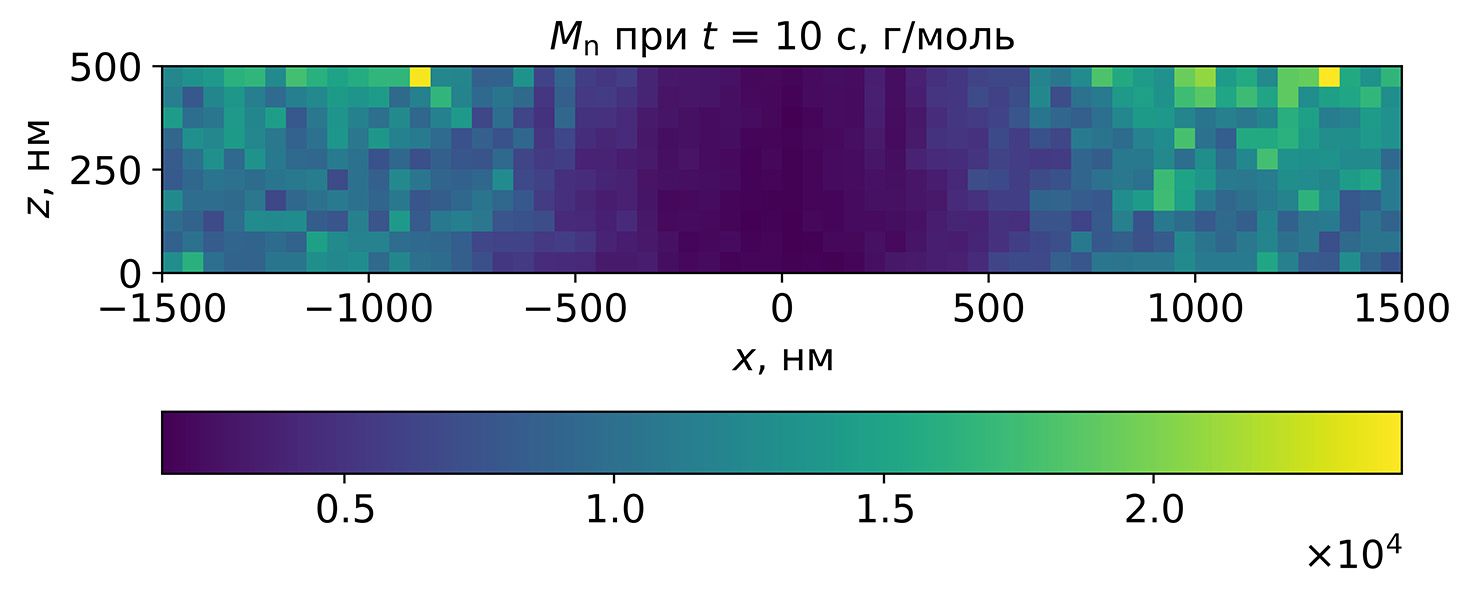
\includegraphics[width=0.7\linewidth]{MW/Mn_hist_10s_straight_200} \\
		\vspace{-3.7em} \text{\hspace{-26em} a)} \vspace{2.7em} \\
		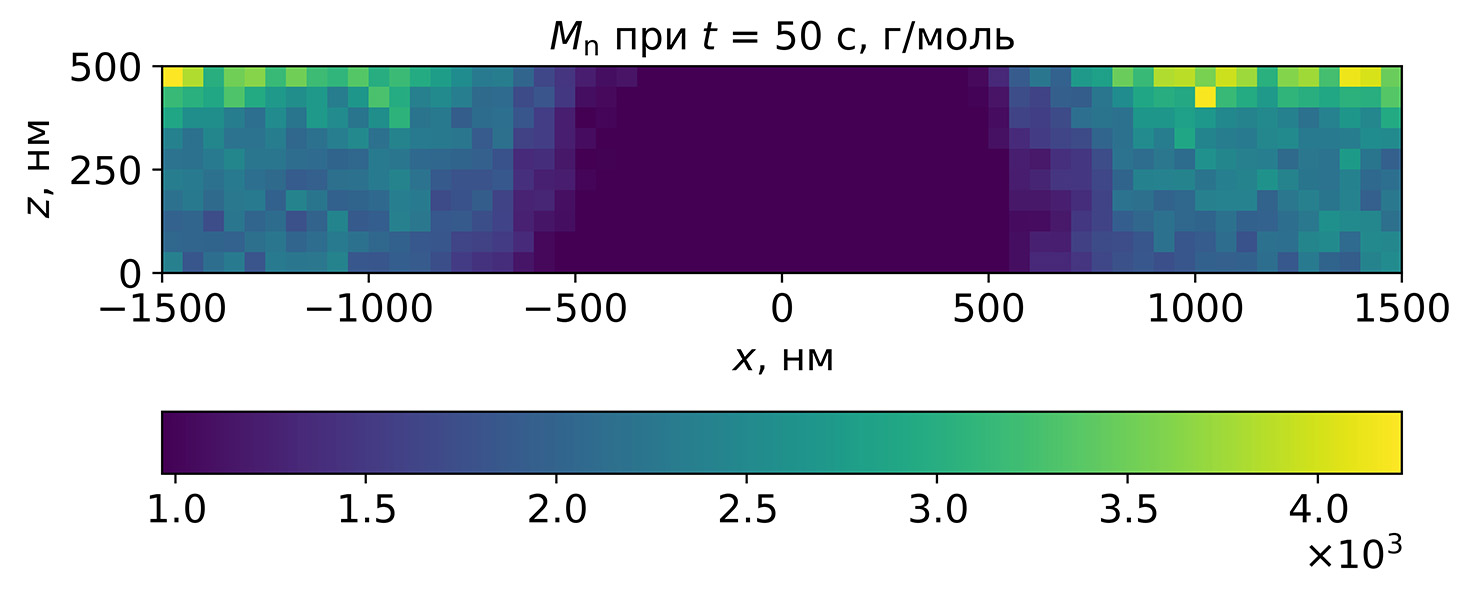
\includegraphics[width=0.7\linewidth]{MW/Mn_hist_50s_straight_200} \\
		\vspace{-3.7em} \text{\hspace{-26em} б)} \vspace{3.7em} \\
	\end{center}
	\vspace{-2.5em}
	\caption{Промоделированные распределения среднечисловой молекулярной массы ПММА при его экспонировании электронным лучом вдоль серии параллельных линий с расстоянием между линиями 3~мкм. Начальная среднечисловая молекулярная масса ПММА составляет примерно 271000, плотность тока экспонирования на единицу длины линии -- 30 пА/см, начальная энергия электронного пучка -- 20 кэВ, толщина слоя ПММА -- 500 нм, температура образца -- 130~$^\circ$C. Время экспонирования составляло 10~с (а) и 50~с (б). Моделирование проводилось в пределах одной линии с периодическими граничными условиями.}
	\label{fig:Mn_hist}
\end{figure}

Моделирование диффузии мономера, образующегося в слое ПММА в процессе деполимеризации, проводилось путем численного решения уравнения диффузии.
Для определения значений коэффициента диффузии мономера в слое ПММА использовались промоделированные распределения среднечисловой молекулярной массы \linebreak ПММА, а также значения и зависимости, приведенные в работах~\cite{Fragala_3_diffusion, Berens_diffusion_Mn}.
Моделирование показало, что за первые несколько секунд процесса СЭЛТР коэффициент диффузии снижается до значений, при которых время диффузии мономера, образующегося за 1~с экспонирования, из слоя ПММА толщиной в несколько сотен нанометров составляет менее 1~с.
Ввиду этого в дальнейшем считалось, что весь мономер, образующийся в процессе деполимеризации, мгновенно покидает слой ПММА, что приводит к образованию микрополостей.

%Распределения вязкости ПММА рассчитывались на основе промоделированных распределений среднечисловой молекулярной массы ПММА, а также значений и зависимостей, приведенных в работе~\cite{Leveder_2010}.
Для моделирования растекания слоя ПММА в процессе СЭЛТР был разработан подход на основе метода конечных элементов.
В данном подходе растекание слоя рассматривалось как процесс эволюции его поверхности под действием сил поверхностного натяжения.
При этом было необходимо учесть, что вследствие неоднородного распределения среднечисловой массы ПММА в процессе СЭЛТР вязкость ПММА также будет иметь неоднородное распределение~\cite{Leveder_2010}.
За счет этого различные участки поверхности слоя ПММА будут двигаться с различной скоростью под действием одной и той же силы.
Для учета этого эффекта вершинам поверхности слоя ПММА приписывались различные значения подвижности, определяющие связь между силой, действующей на вершину, и скоростью вершины.
Соотношение между локальным значением коэффициента вязкости ПММА и подвижностью вершин его поверхности было определено путем моделирования растекания прямоугольных решеток с однородным профилем вязкости аналитическим~\cite{Leveder_2010} и численным~\cite{Brakke_SE} методами.
Для значений коэффициента вязкости в диапазоне \linebreak 10$\pp$--10$^{\text{6}}$ Па$\cdot$с были подобраны значения подвижности вершин поверхности решеток, обеспечивающие соответствие между результатами моделирования, полученными обоими методами.
В результате было установлено, что подвижность вершин поверхности слоя ПММА $\mu$ может быть рассчитана из вязкости ПММА $\eta$ (в Па$\cdot$с) по формуле
\begin{equation}
	\mu \approx \frac{26.14}{\eta}.
\end{equation}
Полученное соотношение позволяло рассчитать значения подвижности для вершин поверхности сплошной структуры в слое ПММА с известным распределением вязкости и в дальнейшем численно промоделировать растекание этой структуры.

Однако, в методе СЭЛТР слой ПММА не является сплошным, и процессы растекания протекают за счет действия сил поверхностного натяжения как на поверхности слоя, так и на границах микрополостей внутри него.
Поэтому при моделировании процессов растекания использовалось приближение, состоящее в преобразовании слоя \linebreak ПММА в сплошную структуру.
Слой ПММА разделялся в плоскости $XY$ на участки размерами 100$\times$100 нм$\pp$, и для каждого участка на основе промоделированного распределения разрывов молекул ПММА и средней длины кинетической цепи при деполимеризации рассчитывались положения и объемы микрополостей (рисунок~\ref{fig:reflow_surface}а).
Далее точки поверхности слоя ПММА, соответствующие середине каждого участка по оси $X$, сдвигались вниз таким образом, чтобы объем призмы, образующейся под поверхностью слоя, был равен суммарному объему микрополостей на этом участке (рисунок~\ref{fig:reflow_surface}б).
Подвижности вершин полученной пилообразной структуры рассчитывались из распределения вязкости ПММА, после чего растекание структуры моделировалось численно в течение нужного промежутка времени.

\begin{figure}[h]
	\begin{minipage}{0.48\textwidth}
		\includegraphics[width=0.9\linewidth]{reflow/reflow_model_a_CIRCLES_4} \\
		\vspace{-28.5ex} \\ \text{\hspace{0em} a}) \\ \vspace{28.5ex}
	\end{minipage}
	\begin{minipage}{0.48\textwidth}
		\includegraphics[width=0.9\linewidth]{reflow/reflow_model_b} \\
		\vspace{-28.5ex} \\ \text{\hspace{-0.1em} б}) \\ \vspace{28.5ex}
	\end{minipage}
	\vspace{-3.5em}
	\caption{Иллюстрация подхода к моделированию растекания слоя ПММА со внутренними микрополостями.}
	\label{fig:reflow_surface}
\end{figure}

Объединение моделей рассеяния электронного пучка, электронно-стимулированных разрывов молекул ПММА, электронно-стимулированной термической деполимеризации ПММА, диффузии мономера и растекания слоя ПММА позволило создать модель модель сухого электронно-лучевого травления резиста.
На ее основе был разработан алгоритм моделирования профиля линии, получаемой методом СЭЛТР при произвольных параметрах процесса.
В данном алгоритме все время экспонирования разделялось на промежутки величиной 1~с, и на каждом промежутке последовательно выполнялись следующие действия:

\begin{enumerate}
	\item Моделирование рассеяния электронного пучка в системе ПММА/Si;
	\item Моделирование электронно-стимулированных разрывов молекул ПММА;
	\item Моделирование термической деполимеризации ПММА;
	\item Определение значений подвижности вершин поверхности слоя ПММА;
	\item Вычисление положений и объемов микрополостей в слое ПММА;
	\item Преобразование слоя ПММА в сплошную пилообразную структуру;
	\item Моделирование растекания пилообразной структуры;
	\item Определение нового положения поверхности слоя ПММА.
\end{enumerate}
По истечении времени экспонирования моделировалось растекание слоя ПММА при охлаждении образца.

\underline{\textbf{В четвертой главе}} приводятся результаты  диссертационной работы.
Описывается верификация разработанной модели сухого электронно-лучевого травления резиста, а также ее применение для определения предельного разрешения метода СЭЛТР.
Помимо этого, разработанная модель используется для исследования влияния флуктуаций параметров процесса СЭЛТР на конечный профиль получаемой линии, а также для определения параметров процесса СЭЛТР для формирования синусоидальных дифракционных и голографических элементов.

Для верификации разработанной модели методом СЭЛТР были получены периодические структуры в слое ПММА на кремниевой подложке.
Экспонирование производилось в рабочей камере растрового электронного микроскопа CAMSCAN S-4, который был модифицирован для возможности нагрева образца, начальная толщина слоя ПММА составляла 500 нм.
Давление в камере микроскопа поддерживалось на уровне 10$^\text{-5}$ мбар, энергия электронного пучка составляла 20 кэВ, диаметр пучка -- \linebreak около 600 нм.
Экспонирование резиста производилось ``в кадр'' (вдоль серии параллельных линий), размеры кадра составляли 2.4$\times$1.9~мм$\pp$, число линий в кадре равнялось 625.
Ток экспонирования $I$ находился в диапазоне 4.56--5.62 нА, время экспонирования $t_\mathrm{exp}$ варьировалось от 100 до 200 с, таким образом, доза экспонирования на единицу длины линии $D_\mathrm{l}$ составляла 3.00--7.38~нКл/см.
Температура подложки образцов при экспонировании $T$ варьировалась от 130 до 150~$^\circ$C, скорость охлаждения подложки после экспонирования составляла около 0.2~$^\circ$C/с.
Профили линий были получены методом атомно-силовой микроскопии с использованием микроскопа Nanopics~2100.

Для снижения требуемого машинного времени моделирование проводилось для участка одной линии длиной 100 нм, влияние соседних линий учитывалось за счет использования периодических граничных условий.
Число разрывов молекул ПММА, локальная среднечисловая молекулярная масса ПММА и объемы микрополостей вычислялись для ячеек размерами 100$\times$100$\times$5 нм$\ppp$ (по осям $X$, $Y$ и $Z$, соответственно).
Для учета стохастической природы алгоритма моделирования для каждого набора параметров экспонирования проводилось 100 независимых моделирований.
Далее на основе 100 полученных профилей рассчитывался усредненный промоделированный профиль (слово ``усредненный'' в дальнейшем будет опускаться).
Сравнение экспериментальных и промоделированных профилей приведено на рисунке~\ref{fig:DEBER_2_profiles}.
Высокая степень воспроизведения экспериментальных профилей указывает на достоверность разработанной модели процесса СЭЛТР.

\begin{figure}[h]
	\begin{minipage}{0.48\textwidth}
		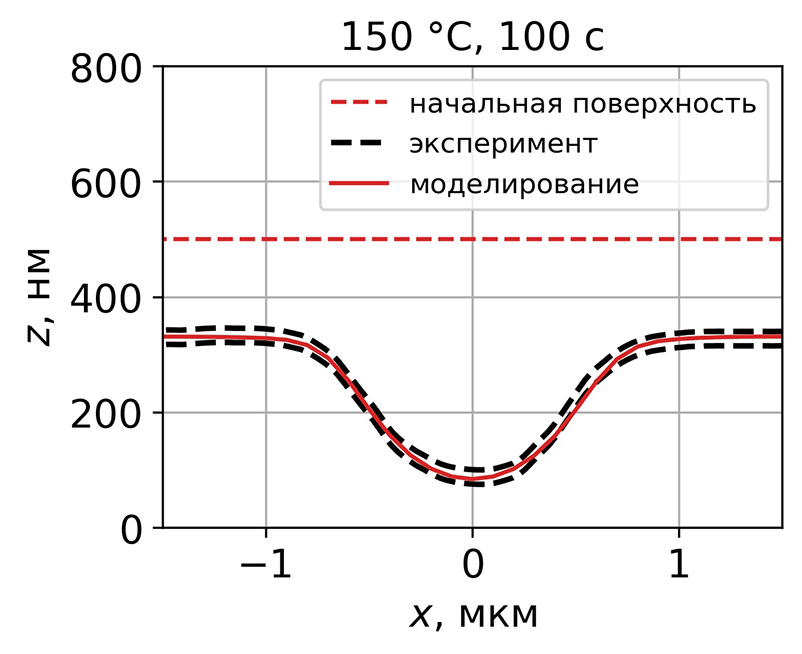
\includegraphics[width=0.9\linewidth]{DEBER_verification/150C_100s_14_FINAL_200} \\
		\vspace{-12em} \\ \text{\hspace{0em} a}) \\ \vspace{12em}
	\end{minipage}
	\begin{minipage}{0.48\textwidth}
		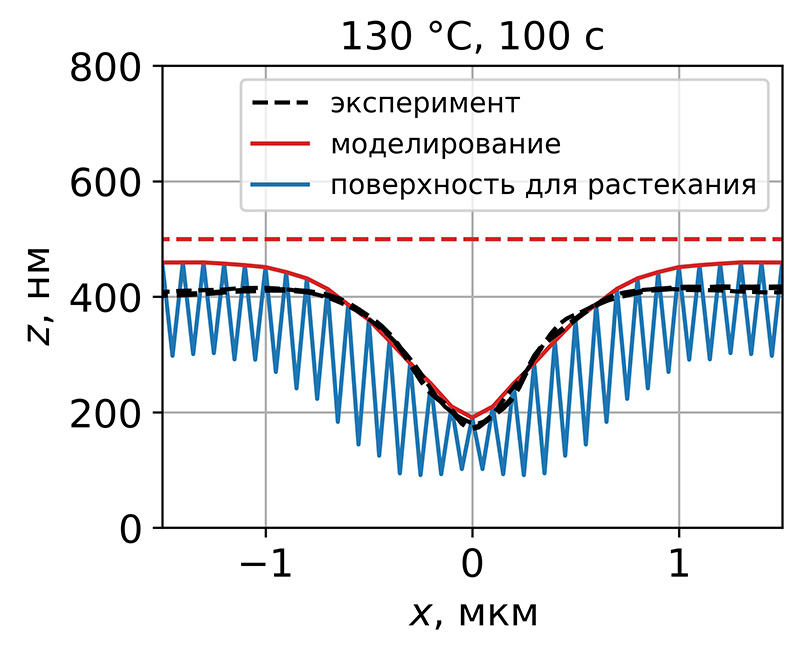
\includegraphics[width=0.9\linewidth]{DEBER_verification/130C_100s_14_FINAL_200} \\
		\vspace{-12em} \\ \text{\hspace{-0.1em} б}) \\ \vspace{12em}
	\end{minipage}
	\vspace{-3.5em}
	\caption{
		Верификация разработанной модели процесса СЭЛТР -- сравнение экспериментальных и промоделированных профилей для следующих условий экспонирования: a) $T$ = 150~$^\circ$C, $t_\mathrm{exp}$ = 100 c, $D_\mathrm{l}$ = 3.00 нКл/см; б) $T$ = 130~$^\circ$C, $t_\mathrm{exp}$ = 100 c, $D_\mathrm{l}$ = 3.12 нКл/см.
		В обоих случаях начальная энергия электронного пучка составляла 20 кэВ, диаметр пучка -- около 600~нм, скорость охлаждения подложки после экспонирования -- примерно 0.2~$^\circ$C/с.
		Черная пунктирная линия обозначает профили, полученные в эксперименте, красная пунктирная линия -- начальное положение поверхности ПММА, синяя линия -- пилообразную поверхность, использовавшуюся при моделировании растекания слоя ПММА со внутренними микрополостями.}
	\label{fig:DEBER_2_profiles}
%	\vspace{1em}
\end{figure}

На основе разработанной модели были выявлены два пути увеличения разрешения метода СЭЛТР.
Во-первых, латеральное разрешение метода может быть увеличено за счет использования узкого высокоэнергетического пучка.
Малый диаметр пучка позволит локализовать большинство разрывов молекул резиста в центре линии, что вызовет интенсивную деполимеризацию, образование микрополостей и снижение вязкости резиста в этой области.
Помимо этого, за счет высокой энергии пучка будет снижено число разрывов на краях линии, вызванных обратно отраженными электронами.
При этом будет необходимо подобрать время экспонирования так, чтобы на момент остывания образца микрополости в центре линии заполнились, а микрополости на краях -- остались незаполненными.
Во-вторых, использование узкого низкоэнергетического пучка также может увеличить латеральное разрешение метода СЭЛТР.
При низкой энергии первичных электронов все разрывы полимерных молекул будут происходить вблизи центра линии за счет относительно небольшой глубины проникновения электронов.
В этом случае микрополости будут формироваться только в ограниченной области вблизи центра линии, что исключит проседание краев линии.
На рисунке~\ref{fig:DEBER_resolution} приведены результаты моделирования профилей, полученных методом СЭЛТР с латеральным разрешением, увеличенным обоими вышеописанными способами.
На основе результатов моделирования было установлено, что минимальная ширина на полувысоте и максимальный угол наклона стенок канавки, получаемой методом СЭЛТР при экспонировании в линию, составляют около 300 нм и 70$^\circ$ соответственно.

\begin{figure}[h]
	\begin{minipage}{0.48\textwidth}
		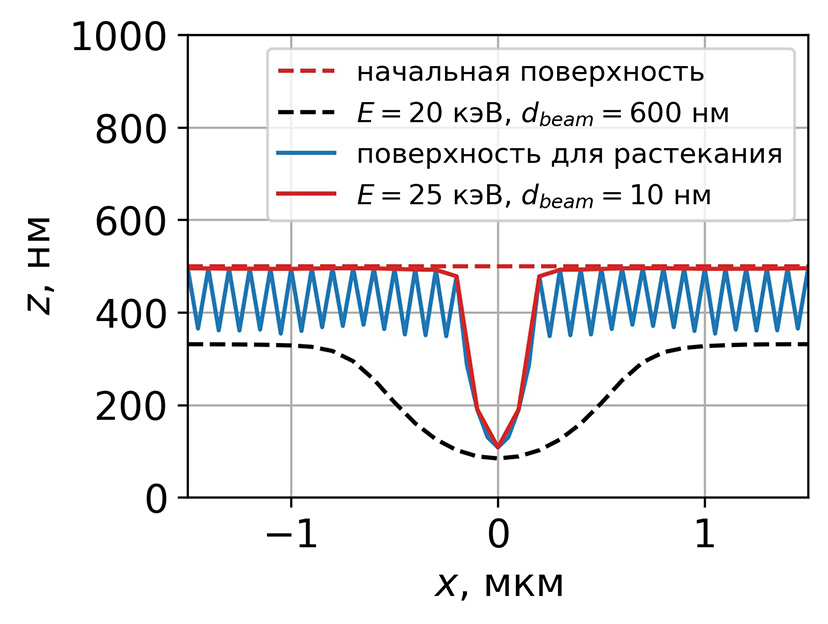
\includegraphics[width=\linewidth]{DEBER_resolution/resolution_25_um_200} \\
		\vspace{-28.7ex} \\ \text{\hspace{0em} a}) \\ \vspace{28.7ex}
	\end{minipage}
	\begin{minipage}{0.48\textwidth}
		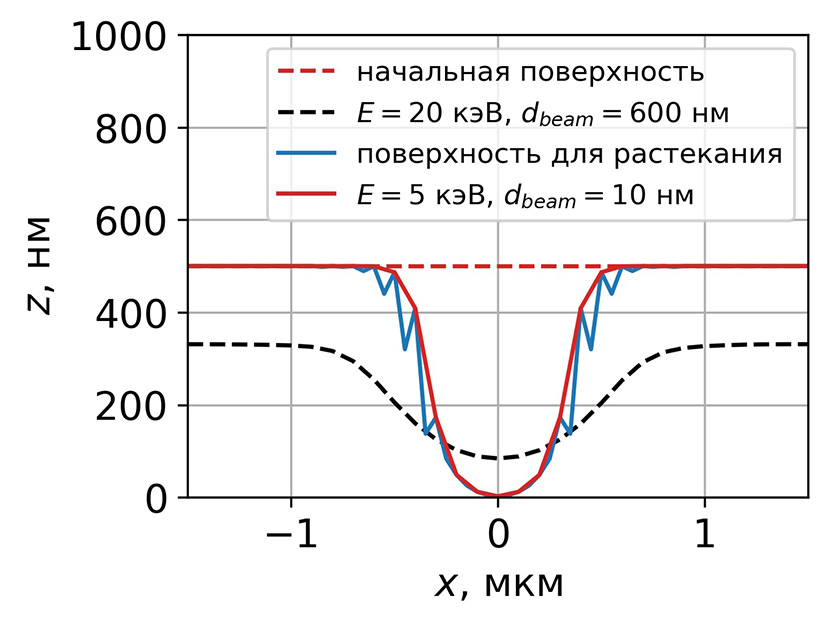
\includegraphics[width=\linewidth]{DEBER_resolution/resolution_5_um_200} \\
		\vspace{-28.7ex} \\ \text{\hspace{-0.1em} б}) \\ \vspace{28.7ex}
	\end{minipage}
	\vspace{-3.5em}
	\caption{
		Моделирование профилей, полученных методом СЭЛТР при использовании узкого пучка с энергией 25 кэВ (а) и 5 кэВ (б).
		Диаметр пучка составлял 10 нм, температура образцов -- 150~$^\circ$C/с, начальная толщина слоя ПММА -- 500 нм.
		Экспонирование производилось вдоль одиночной линии, плотность тока экспонирования на единицу длины линии составляла 30~пА/см, скорость охлаждения образцов -- 10~$^\circ$C/с.}
	\label{fig:DEBER_resolution}
\end{figure}

Разработанный алгоритм моделирования профиля линии, получаемой методом СЭЛТР, также был использован для исследования влияния флуктуаций параметров экспонирования на профиль линии.
Это позволило сформулировать требования к стабильности параметров экспонирования в методе СЭЛТР: для получения необходимого профиля флуктуации энергии пучка, тока экспонирования и температуры образца должны составлять не более 0.5~кэВ, 0.1~нА и 1~$^\circ$C соответственно.
Такие флуктуации параметров экспонирования приводят к флуктуациям высоты точек промоделированного профиля, сопоставимым со среднеквадратичным отклонением высоты точек при моделировании (около 2 нм).
Максимально допустимая флуктуация скорости охлаждения образца, определенная аналогичным образом, составляет 0.1~$^\circ$C/с.

Проведенные эксперименты показали, что при экспонировании резиста в методе СЭЛТР ``в кадр'' профиль получаемого рельефа имеет волнообразную форму.
Вследствие этого целесообразным являлось изучение возможности использования метода СЭЛТР для формирования синусоидальных голографических решеток, широко применяющихся в оптике.
На основании результатов моделирования можно заключить, что методом СЭЛТР в слое ПММА могут быть получены синусоидальные решетки с плотностью штрихов до 2000 1/мм.
Как показано на рисунке~\ref{fig:DEBER_holo_2um}, синусоидальный профиль рельефа может быть получен как при наличии микрополостей в слое ПММА на момент остывания образца (рисунки~\ref{fig:DEBER_holo_2um}a, \ref{fig:DEBER_holo_2um}б), так и при их отсутствии (рисунки~\ref{fig:DEBER_holo_2um}в, \ref{fig:DEBER_holo_2um}г).
При этом среднеквадратичное отклонение точек промоделированных профилей от графика функции синус составляет менее 5\% от глубины решетки.
Полученные в ПММА синусоидальные решетки могут быть в дальнейшем покрыты металлом или перенесены в металл путем травления в реакторе индуктивно-связанной плазмы~\cite{Bruk_2016_mee}, что может быть использовано для формирования отражательных синусоидальных голографических решеток.

\begin{figure}[h!]
	\begin{minipage}{0.48\textwidth}
		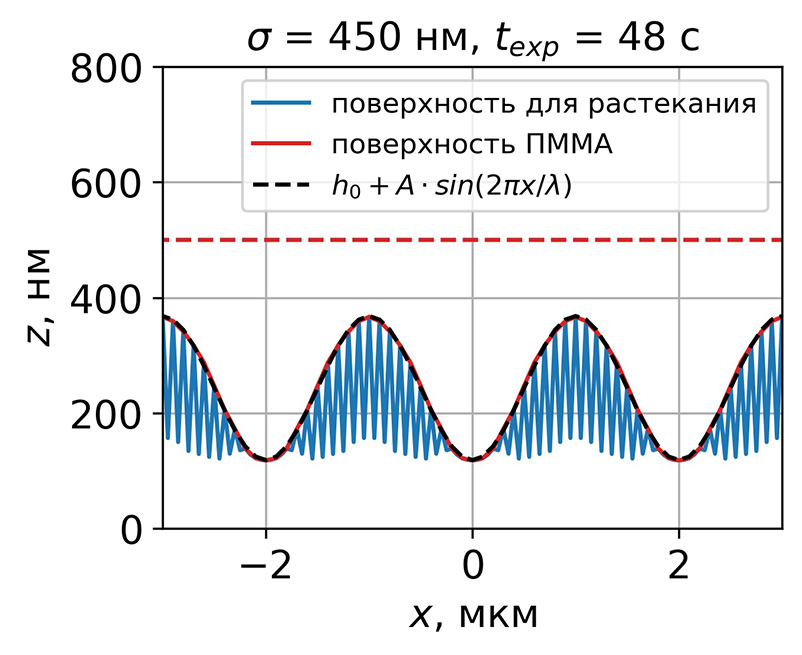
\includegraphics[width=0.9\linewidth]{DEBER_holo/2_um/holo_1C_s450_48s_um_200} \\
		\vspace{-12em} \\ \text{\hspace{0em} a}) \\ \vspace{12em}
	\end{minipage}
	\begin{minipage}{0.48\textwidth}
		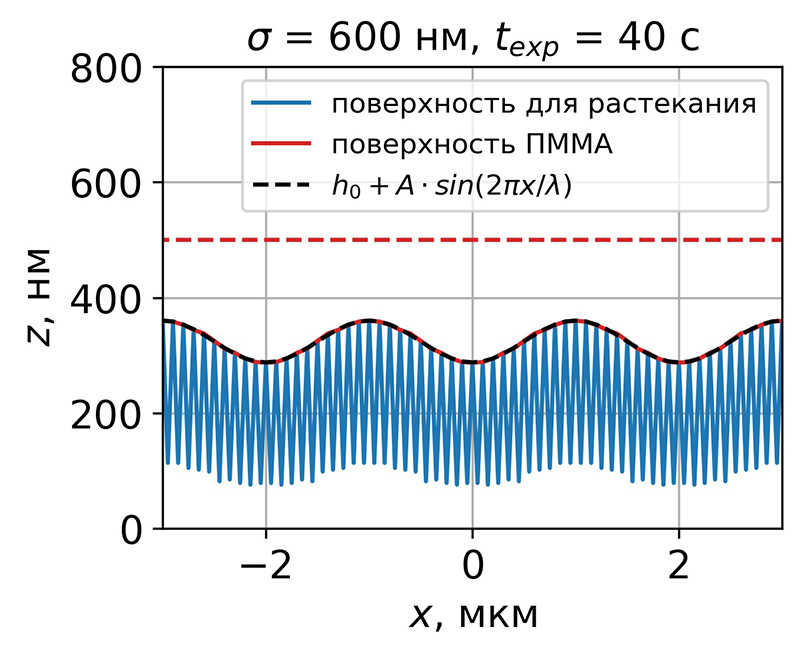
\includegraphics[width=0.9\linewidth]{DEBER_holo/2_um/holo_1C_s600_40s_um_200} \\
		\vspace{-12em} \\ \text{\hspace{-0.1em} б}) \\ \vspace{12em}
	\end{minipage}
	
	\vspace{-3.5em}
	
	\begin{minipage}{0.48\textwidth}
		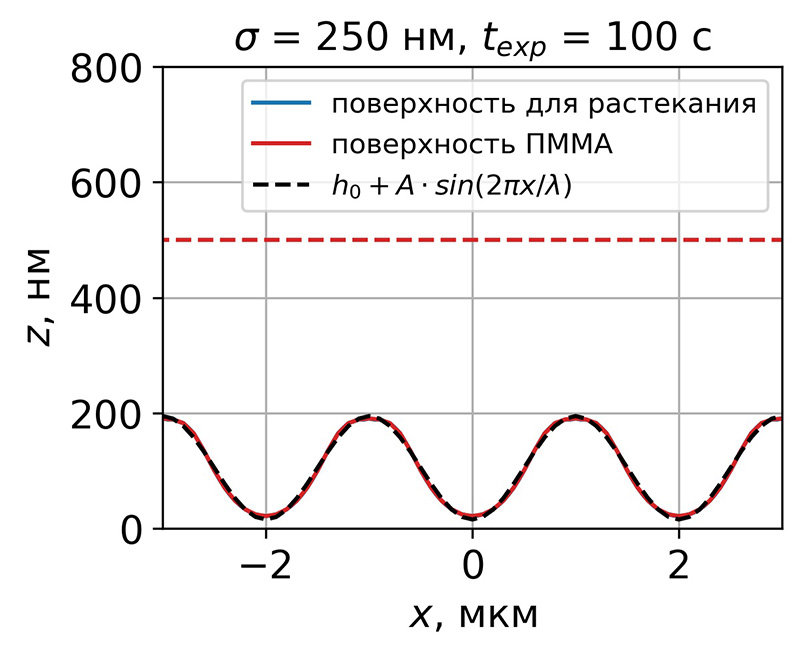
\includegraphics[width=0.9\linewidth]{DEBER_holo/2_um/holo_10C_s250_100s_um_200} \\
		\vspace{-12em} \\ \text{\hspace{0em} в}) \\ \vspace{12em}
	\end{minipage}
	\begin{minipage}{0.48\textwidth}
		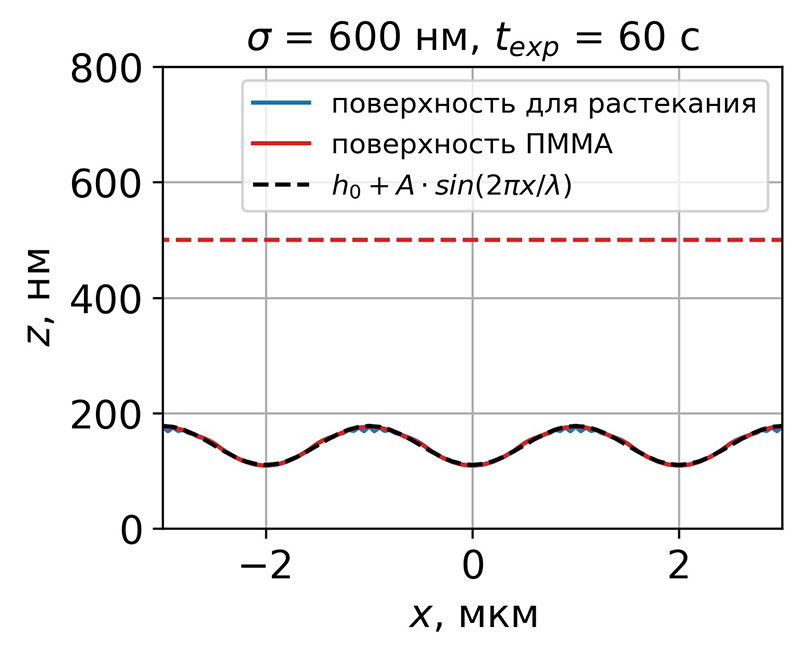
\includegraphics[width=0.9\linewidth]{DEBER_holo/2_um/holo_1C_s600_60s_um_200} \\
		\vspace{-12em} \\ \text{\hspace{-0.1em} г}) \\ \vspace{12em}
	\end{minipage}
	\vspace{-3.5em}
	\caption{Промоделированные синусоидальные профили с пространственным периодом $\lambda$ = 2~мкм, полученные методом СЭЛТР в слое ПММА с начальной толщиной 500 нм. Температура образцов при экспонировании составляла 150~$^\circ$C, плотность тока экспонирования на единицу длины линии -- 30 пА/см, начальная энергия электронного пучка -- 20 кэВ, распределение плотности тока в пучке считалось нормальным со среднеквадратичным отклонением $\sigma$. Значения $\sigma$ и $t_\mathrm{exp}$ были подобраны для получения синусоидального профиля. После экспонирования образец а) охлаждался со скоростью 10~$^\circ$C/с, образцы б)-г) -- со скоростью 1~$^\circ$C/с. Черная пунктирная линия обозначает аппроксимацию промоделированного профиля функцией синус.}
	\label{fig:DEBER_holo_2um}
\end{figure}

Приведенные выше промоделированные профили относятся к структурам, получаемым методом СЭЛТР при экспонировании вдоль серии параллельных линий либо вдоль одиночной линии.
Однако, при моделировании может быть заложено произвольное распределение плотности тока по области экспонирования (рисунок~\ref{fig:DEBER_multibeam}).
За счет этого разработанные в данной работе модель СЭЛТР и алгоритм моделирования профиля линии, получаемой в этом процессе, могут использоваться при определении параметров для формирования методом СЭЛТР необходимого профиля.
В самом деле, для получения методом СЭЛТР рельефа, профиль которого согласуется с предельным разрешением метода, параметры экспонирования и последующего охлаждения образца могут быть подобраны путем многократного моделирования конечного профиля с учетом выявленных особенностей метода.

\begin{figure}[h]	
	\begin{minipage}{0.48\textwidth}
		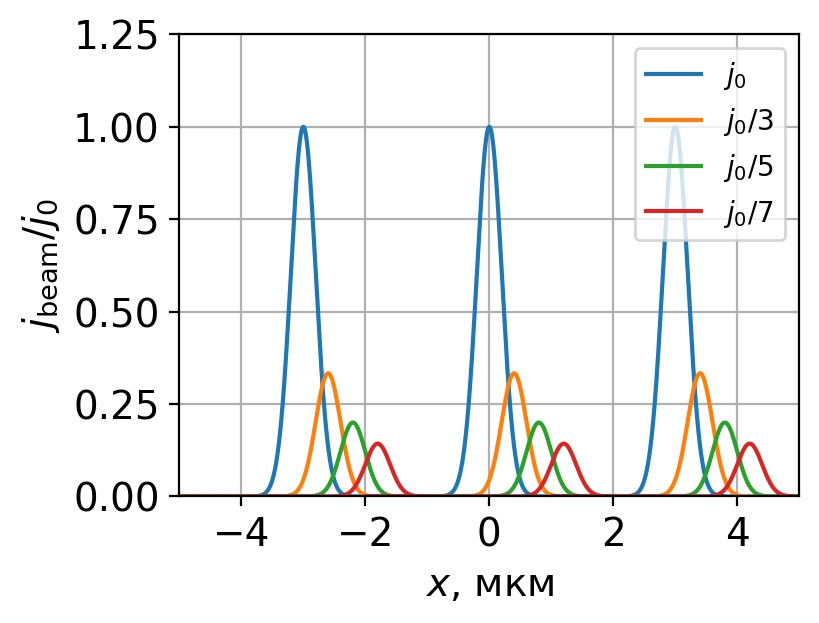
\includegraphics[width=0.9\linewidth]{DEBER_asymmetric/asymmetric_beam_200} \\
		\vspace{-12em} \\ \text{\hspace{0em} а}) \\ \vspace{12em}
	\end{minipage}
	\begin{minipage}{0.48\textwidth}
		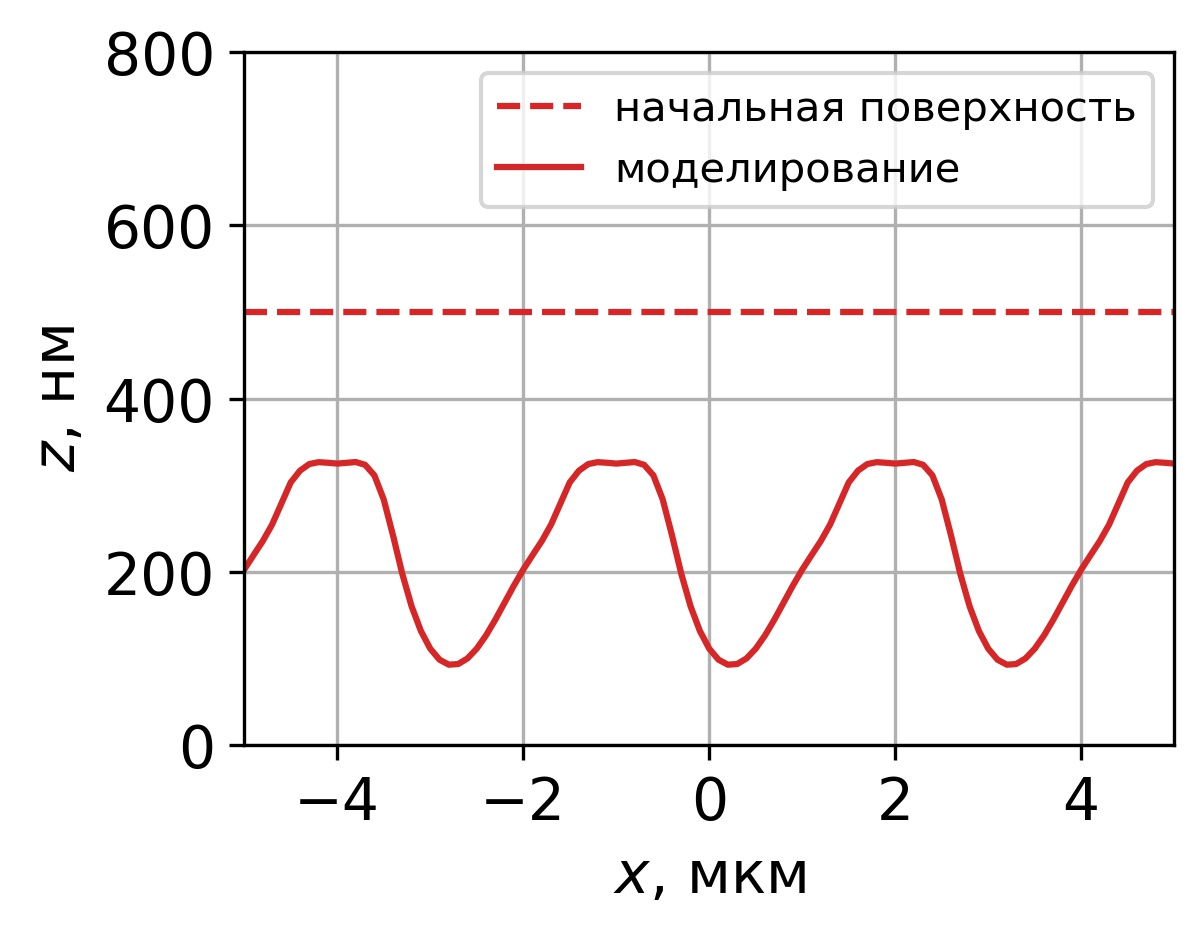
\includegraphics[width=0.9\linewidth]{DEBER_asymmetric/asymmetric_profile_200} \\
		\vspace{-12em} \\ \text{\hspace{-0.1em} б}) \\ \vspace{12em}
	\end{minipage}
	\vspace{-3.5em}
	\caption{Демонстрация возможностей разработанного алгоритма -- моделирование профилей (б), полученных в слое ПММА с начальной толщиной 500~нм методом СЭЛТР при экспонировании по области с плотностью тока в пучке, описывающейся суммой нескольких функций Гаусса (a). Температура образца при экспонировании -- 150~$^\circ$C/с, время экспонирования -- 100 с, плотность тока экспонирования на единицу длины линии -- 30 пА/см.}
	\label{fig:DEBER_multibeam}
	\vspace{2em}
\end{figure}
